% !TEX root = ../thesis.tex

\chapter{案例分析}
流行的数据处理框架比如Hadoop,Spark,Naiad或Hyracks都由托管式语言开发,例如Java,C\#,或Scala。JVM提供的内存自动管理——垃圾收集器(GC)为开发者提供便利。然而,垃圾收集开销是非常大的,GC在这些大数据系统中,可占据高达50\%的执行时间,严重损害了系统的性能。

GC执行缓慢的一个关键原因是大数据系统中的对象特征不匹配传统GC设计使用的启发式算法。在这一章,我们分析一个针对大数据系统中对象行为不匹配的解决方案——Yak。Yak能够智能地适应大数据系统的特性,因此,可以有效地管理在这些大数据系统中存在的大量对象。

我们首先在4.1节介绍Yak的研究思路,然后在4.2节分析该系统的局限性。


\section{研究思路}
\subsection{数据特征不匹配}

传统的分代GC都是基于“已存在时间越短的对象越容易被回收”的假设进行设计的。该假设适用于产生大量短暂临时数据的应用程序,对于这些应用来说, 传统分代GC是有效的——GC扫描一小部分堆就能够回收足够多的内存。但是,大数据应用程序的数据特征与传统分代GC假设不同,这种特征可以概括为两条路径,两种假设。

一个典型的大数据处理框架通常存在控制路径和数据路径的明显区别。控制路径有复杂的执行逻辑(例如管理和调度集群,建立master node和worker node之间的通信);数据路径主要包括可以连接到一个数据处理管道的数据操作功能(数据分区、Join或Aggregate、用户定义数据功能、Map或Reduce等)。
\begin{figure}[h]
    \centering
    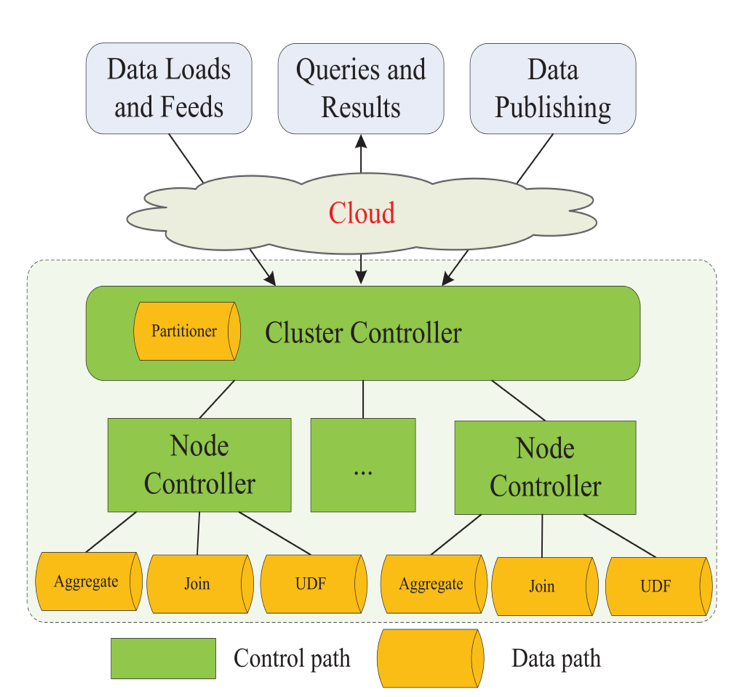
\includegraphics[width=12cm,height=8cm]{figure/two_Path.png}
    \caption{大数据框架架构}
    \label{img1}
\end{figure}
这两条路径遵循不同的对象生命特征,如图\ref{img1}:控制路径上的对象数量小,存活时间短,生命周期符合分代特征,对它们使用传统的分代GC是合理的;而在数据路径上的对象,它们的生命周期呈现出完全不同的时域(epoch)特征(时域特征指的是一组对象在同一时间被创建,在经历一段较长的程序执行时间后才被同时回收的特征),所以不适合采用传统GC。


这种不匹配会导致传统分代GC在数据密集型应用程序中的性能瓶颈。因为创建的对象寿命较长,GC的大部分精力都花费在跟踪巨大数量的对象,而不能及时回收内存。 

两条路径,两种假设启发了一种混合内存管理器——用两种不同的方式管理两种路径对象。对于具有时域特征的数据对象提出更加合适的内存管理方式,同一个时域创建的对象分配在同一个内存区域,同时进行内存回收。

\subsection{设计与实现}
\begin{figure}[h]
    \centering
    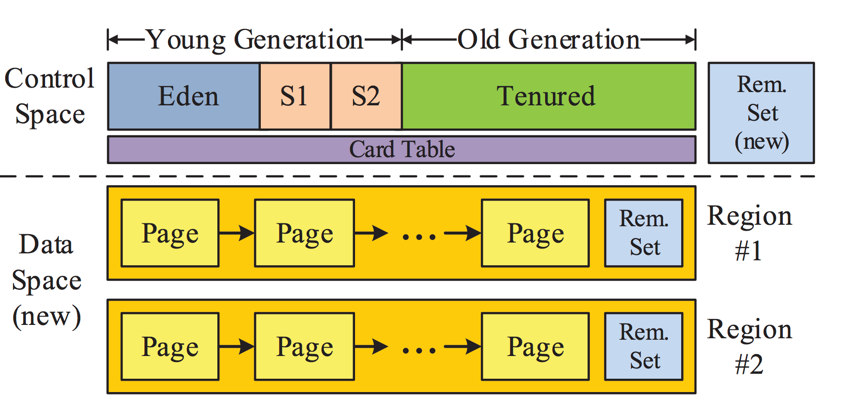
\includegraphics[width=12cm,height=7cm]{figure/layout.png}
    \caption{
       Yak内存分配结构
    }
    \label{img3}
\end{figure}

Yak的高层想法是基于明确区分的控制路径和数据路径,把堆分成一个小的控制空间(CS)和一个更大的数据空间(DS), 并使用不同的机制来管理这些空间,如图\ref{img3},控制空间又被划分为新生代、老生代,采用传统的分代内存管理方法;数据空间则由多个内存域(region)组成,采用基于内存域的内存管理方法。

{\bfseries 问题1:何时创建和释放内存域?}

一个时域代表着一段程序的执行。当一个时域开始时,一个内存域被创建;当一个时域结束时,一个内存域被回收。一个内存域储存对应时域创建的所有对象。一个时域可以是用户自定义的,通过注释的方式实现。举例来说,在Hadoop中,一个用户定义的Map任务被$setup()$和$cleanup()$两个接口调用建立和关闭,开发者可以对这个两个调用的代码进行注释,从而定义一个时域。

为了建立统一的注释,Yak提供了一对用户注释,$epoch\_start()$ 和$epoch\_end()$,这两个注释在运行时被转换成两个本地函数调用,来提醒JVM一个时域的开始和结束。标注这些注释需要的手动工作开销是很小的。即使是新手,没有太多的系统知识,也可以很容易地找到并注释时域。Yak保证执行正确性,当然,时域标注的位置会影响性能:如果一个时域内的对象有不同的寿命,那这些对象会在时域结束后被复制,增加开销。

通常情况下,大数据框架中的系统调用已经具备了很好的时域特性,一旦创建了托管堆(在JVM的启动时期),会保留一系列虚拟地址作为DS。每个时域对应一个内存域,由一组固定长度的内存页组成。

在实践中,需要考虑关于时域概念的更多问题,其中一个是关于时域的嵌套关系。时域嵌套是指在执行的任何时刻,可能会有多个时域,为获得性能优势,Yak支持时域嵌套——内部时域不可达对象可在外部时域结束之前被回收,避免了内存增长过快而造成的内存占用。具体来说,如果一个正在运行的时域间执行$epoch\_start()$,一个新时域开始,创建一个新的内存域,成为上个时域的子时域。所有后续对象分配在子时域,直到遇到一个$epoch\_end()$。

另一个问题是,当多个线程同时执行数据处理代码的相同片段时,如何创建内存域。Yak为每个时域的动态实例创建内存域。当两个线程执行同一时域代码的相同片段时,他们获得自己的内存域而无需考虑同步问题。


\begin{figure}[h]
    \centering
    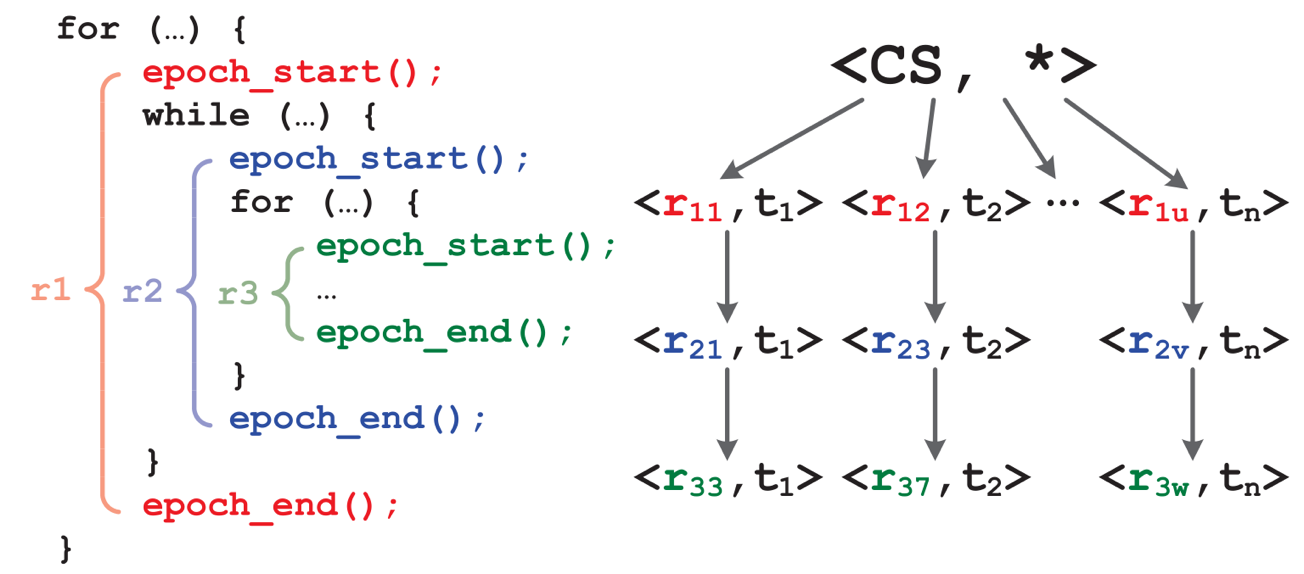
\includegraphics[width=12cm,height=7cm]{figure/epoch.png}
    \caption{
        region的一个例子:(a)一个简单的程序被多个线程执行的过程,(b)对应产生的内存域结构
    }
    \label{img2}
\end{figure}
在执行的任何时刻,可能会有多个时域,因此存在着多个内存域。基于嵌套关系,这些内存域是有一定顺序的,形成半格结构,如\ref {img2}所示,半格上的每个节点是<$r_{ij}$,$t_k$>形式的内存域,$r_{ij}$表示时期$r_i$的第$j$次执行,$t_k$表示线程。例如,区域<$r_{21}$,$t_1$>是<$r_{11}$,$t_1$>的子节点,因为在程序中,时域$r_2$是嵌套在$r_1$中的,并且执行线程相同,都是$t_1$。当被不同的线程执行时,两个时域(例如<$r_{11}$,$t_1$>和<$r_{12}$,$t_2$>)是并发的。

{\bfseries 第二个问题:如何正确并且高效地释放内存域?}

少量的对象存活时间可能比他们所处的时域存在时间长,这些存活对象必须在GC时被标识,并且迁移到安全的空间。Yak必须自动完成两项关键任务:(1)标识存活对象,(2)迁移存活对象。

对于第一项任务,Yak使用高效的算法来追踪跨内存域/空间的引用,并在运行时为每个内存域记录所有的传入引用。在内存域释放之前,Yak将这些引用作为根集合,以计算内存域中迁移对象的传递闭包。

对于第二项任务,对于每个存活对象O,Yak将O重定位到一个活内存域。为了实现这个目标,Yak标识每个传入的对O的跨内存域/跨空间引用的源内存域,并将其进行$join$操作,以在内存域半格上找到最小上界。例如,在图\ref {img2}中,对<$r_{21}$,$t_1$>和<$r_{11}$,$t_1$>进行$join$,返回<$r_{11}$,$t_1$>。若$join$了任意两个并发的区域,则返回到CS。直观地说,如果O有来自父区域和祖父区域的引用,则O应当被移动到祖父区域,如果O有来自两个不同的线程的引用,则必须被移动到CS。

在释放期间,如果其它线程访问将迁移对象的传递闭包,可能会导致不完全闭包。另外,当其他行程运行时,不能并发地移动对象,否则可能会引起数据竞争。为此,Yak使用轻量级的“stop-the-word”处理,以保证在释放时是线程安全的。当一个线程到达时域结束期,Yak暂停所有正在运行的线程,扫描它们的栈,计算释放内存域内所有潜在活对象的闭包。在其它的线程恢复前,将这些对象移动到各自的目标内存域。

Yak在Oracle的JVM OpenJDK 8 (build 25.0-b70)中实现。除了基于时域的技术,还修改了两个JIT编译器(C1和Opto),解释器,对象/堆布局,和Parallel Scavenge收集器,以管理CS。




\section{局限性}


\subsection{写障碍瓶颈}

\begin{figure}[h]
    \centering
    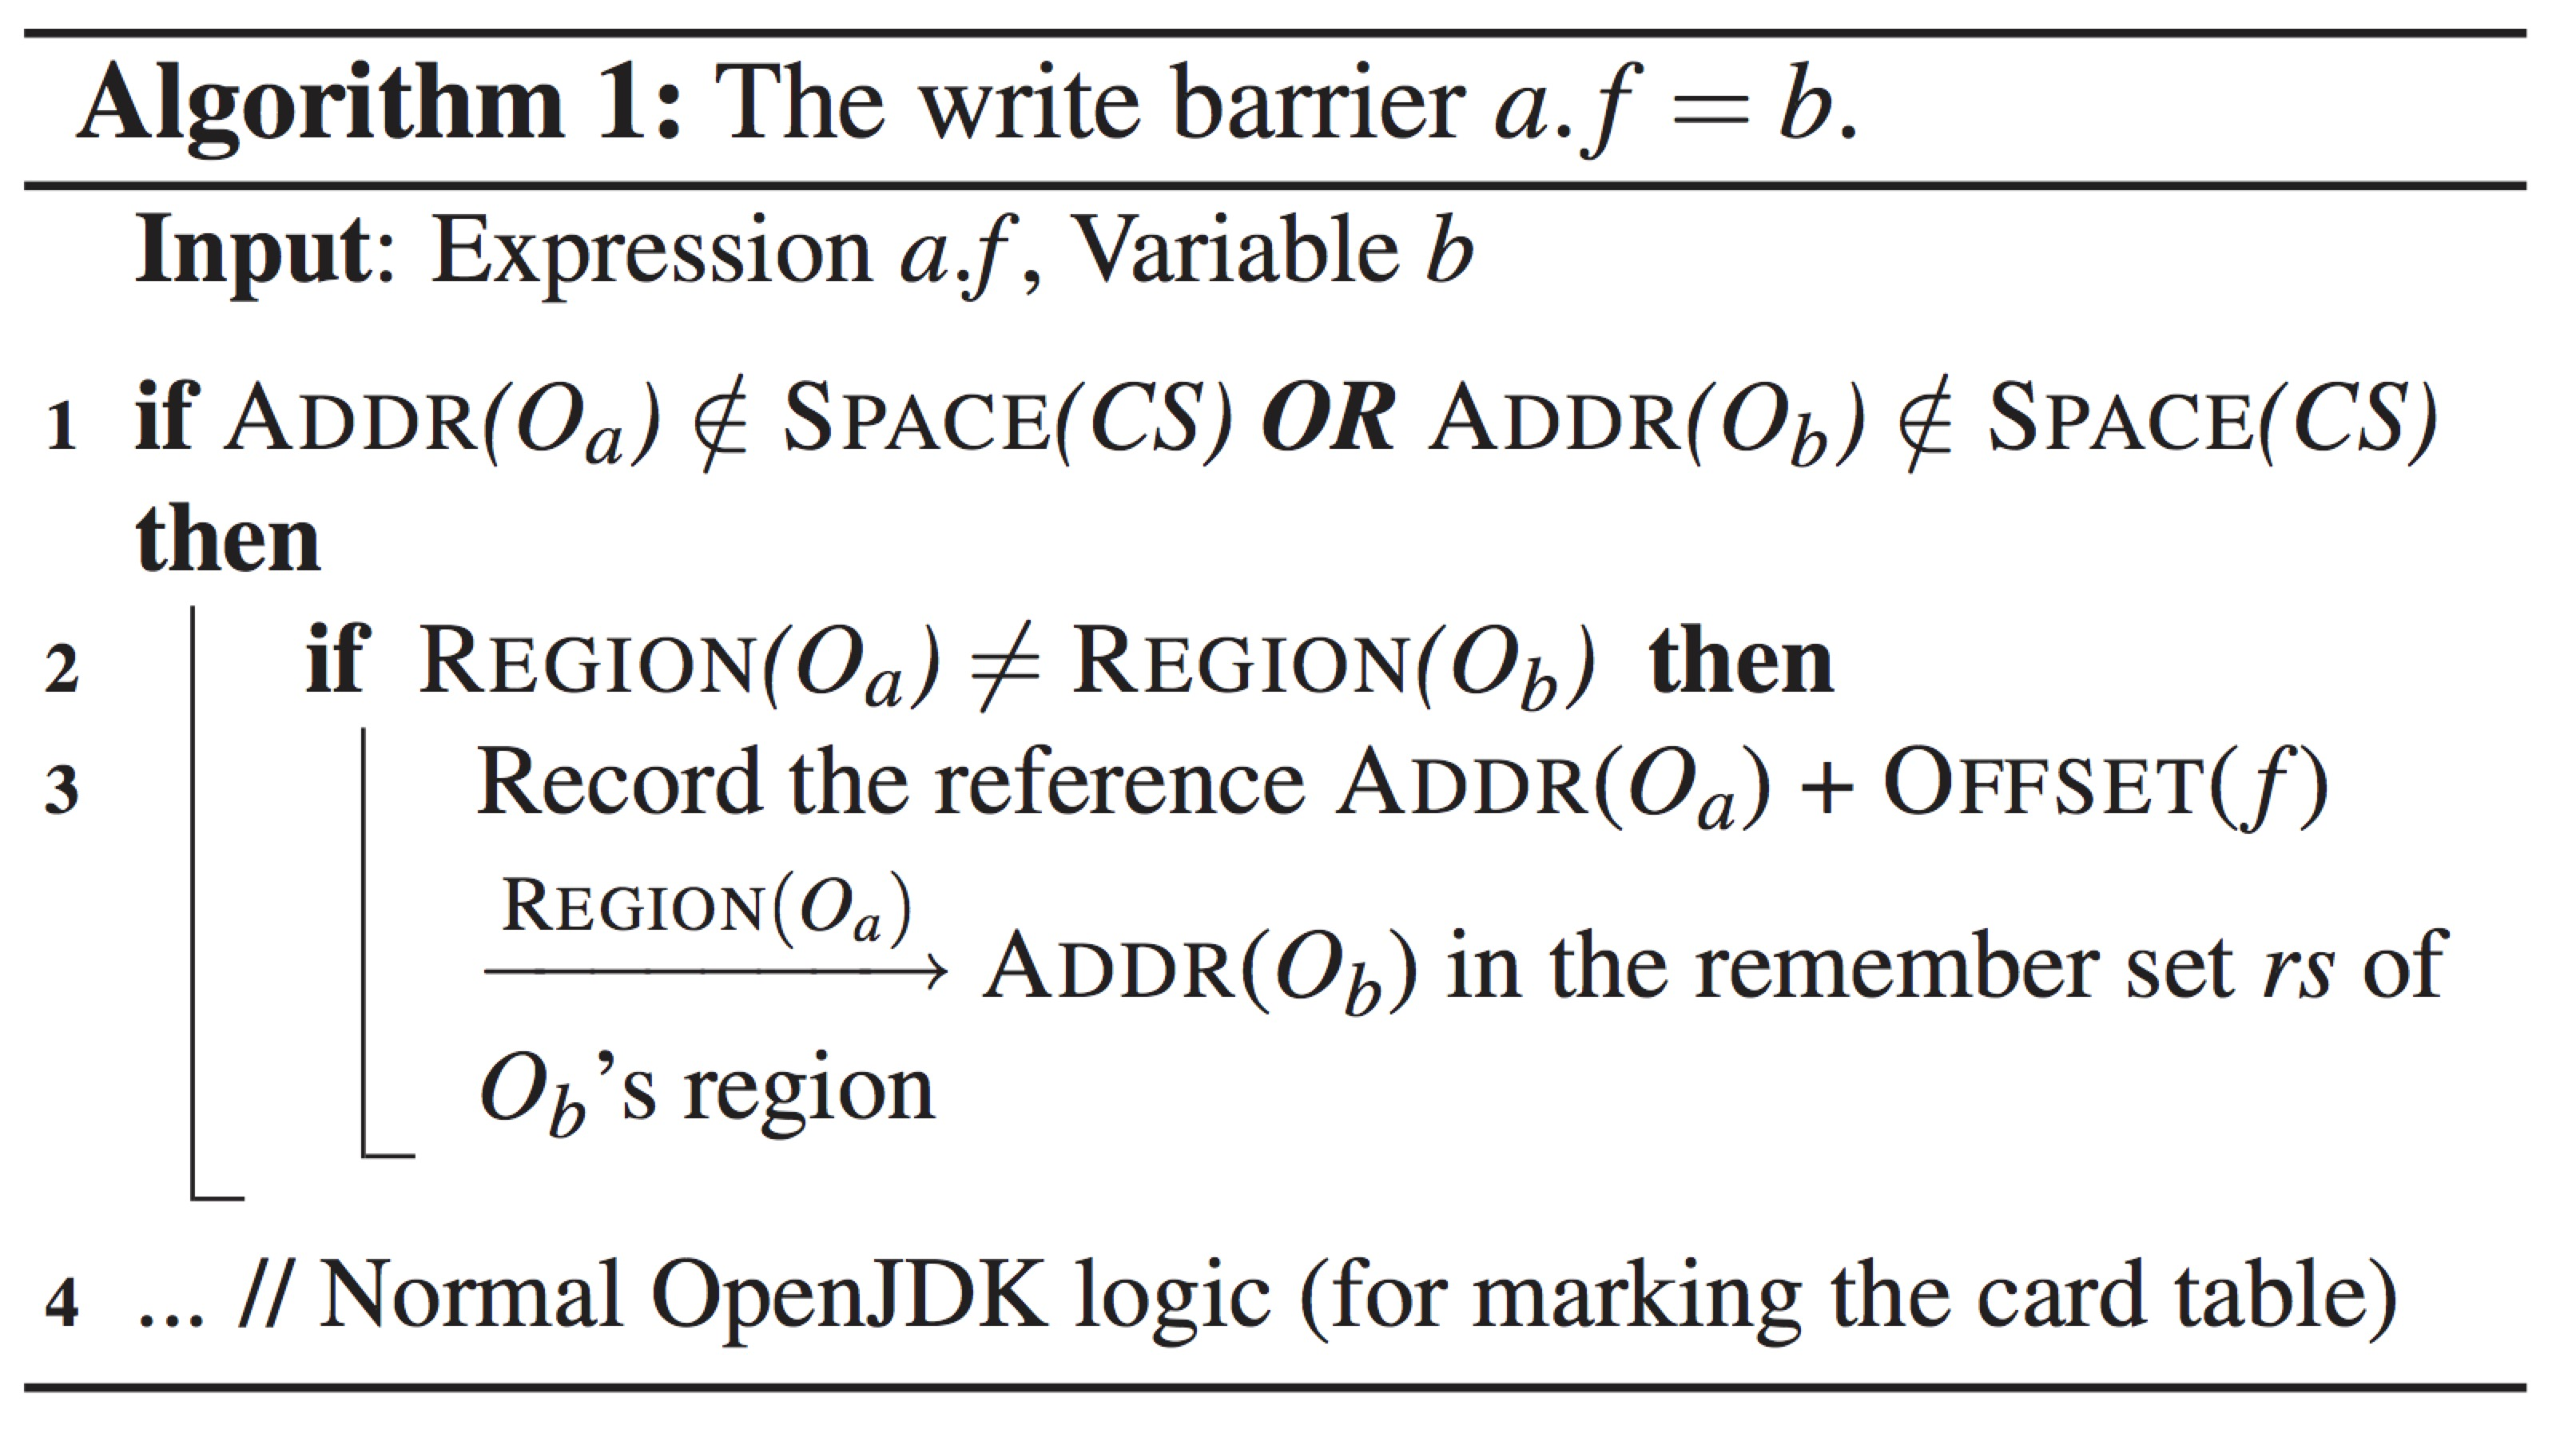
\includegraphics[width=12cm,height=7cm]{figure/algorithm1.jpg}
    \caption{
        算法1:写屏障算法
    }
    \label{algorithm1}
\end{figure}
Yak需要有效地跟踪所有内存域/空间之间的引用。Yak通过三个步骤实现跟踪。首先,Yak将4字节字段(re)添加到每个对象的头部空间来记录对象所属的内存域信息。对象重新分配后,其头部字段更新为相应的内存域ID。CS用一个特殊的ID来表示。然后,Yak修改写障碍(例如,一小段代码增加引用a.f=b,会被写障碍捕获)来检测和记录基于堆的内存域/空间引用,修改后的算法如图\ref{algorithm1}所示。

当对象a新增对对象b的引用,这个引用会被写障碍捕获,将引用关系存储到b所属内存域的记忆集(remember set)中去。

最后,当一个时域结束,Yak通过记忆集来追踪存活对象。

Yak通过写障碍来帮助追踪内存域/空间之间的引用,写障碍本身增加了开销。为了了解写障碍的开销,作者手动修改了GraphChi的执行引擎,强迫载荷滑动碎片和执行更新线程执行写障碍。这对线程序列化产生影响,使程序顺序化。对于GraphChi的三个项目,突变时间(例如non-pause时间)总体增长了24.5\%,这表明写障碍是主要的瓶颈。

现有的GC都通过手工编写/优化汇编代码来实现写障碍。Yak还没有相关的优化,我们希望能够通过优化汇编代码来降低写障碍的开销。


\subsection{适用性局限}
\begin{figure}[h]
    \centering
    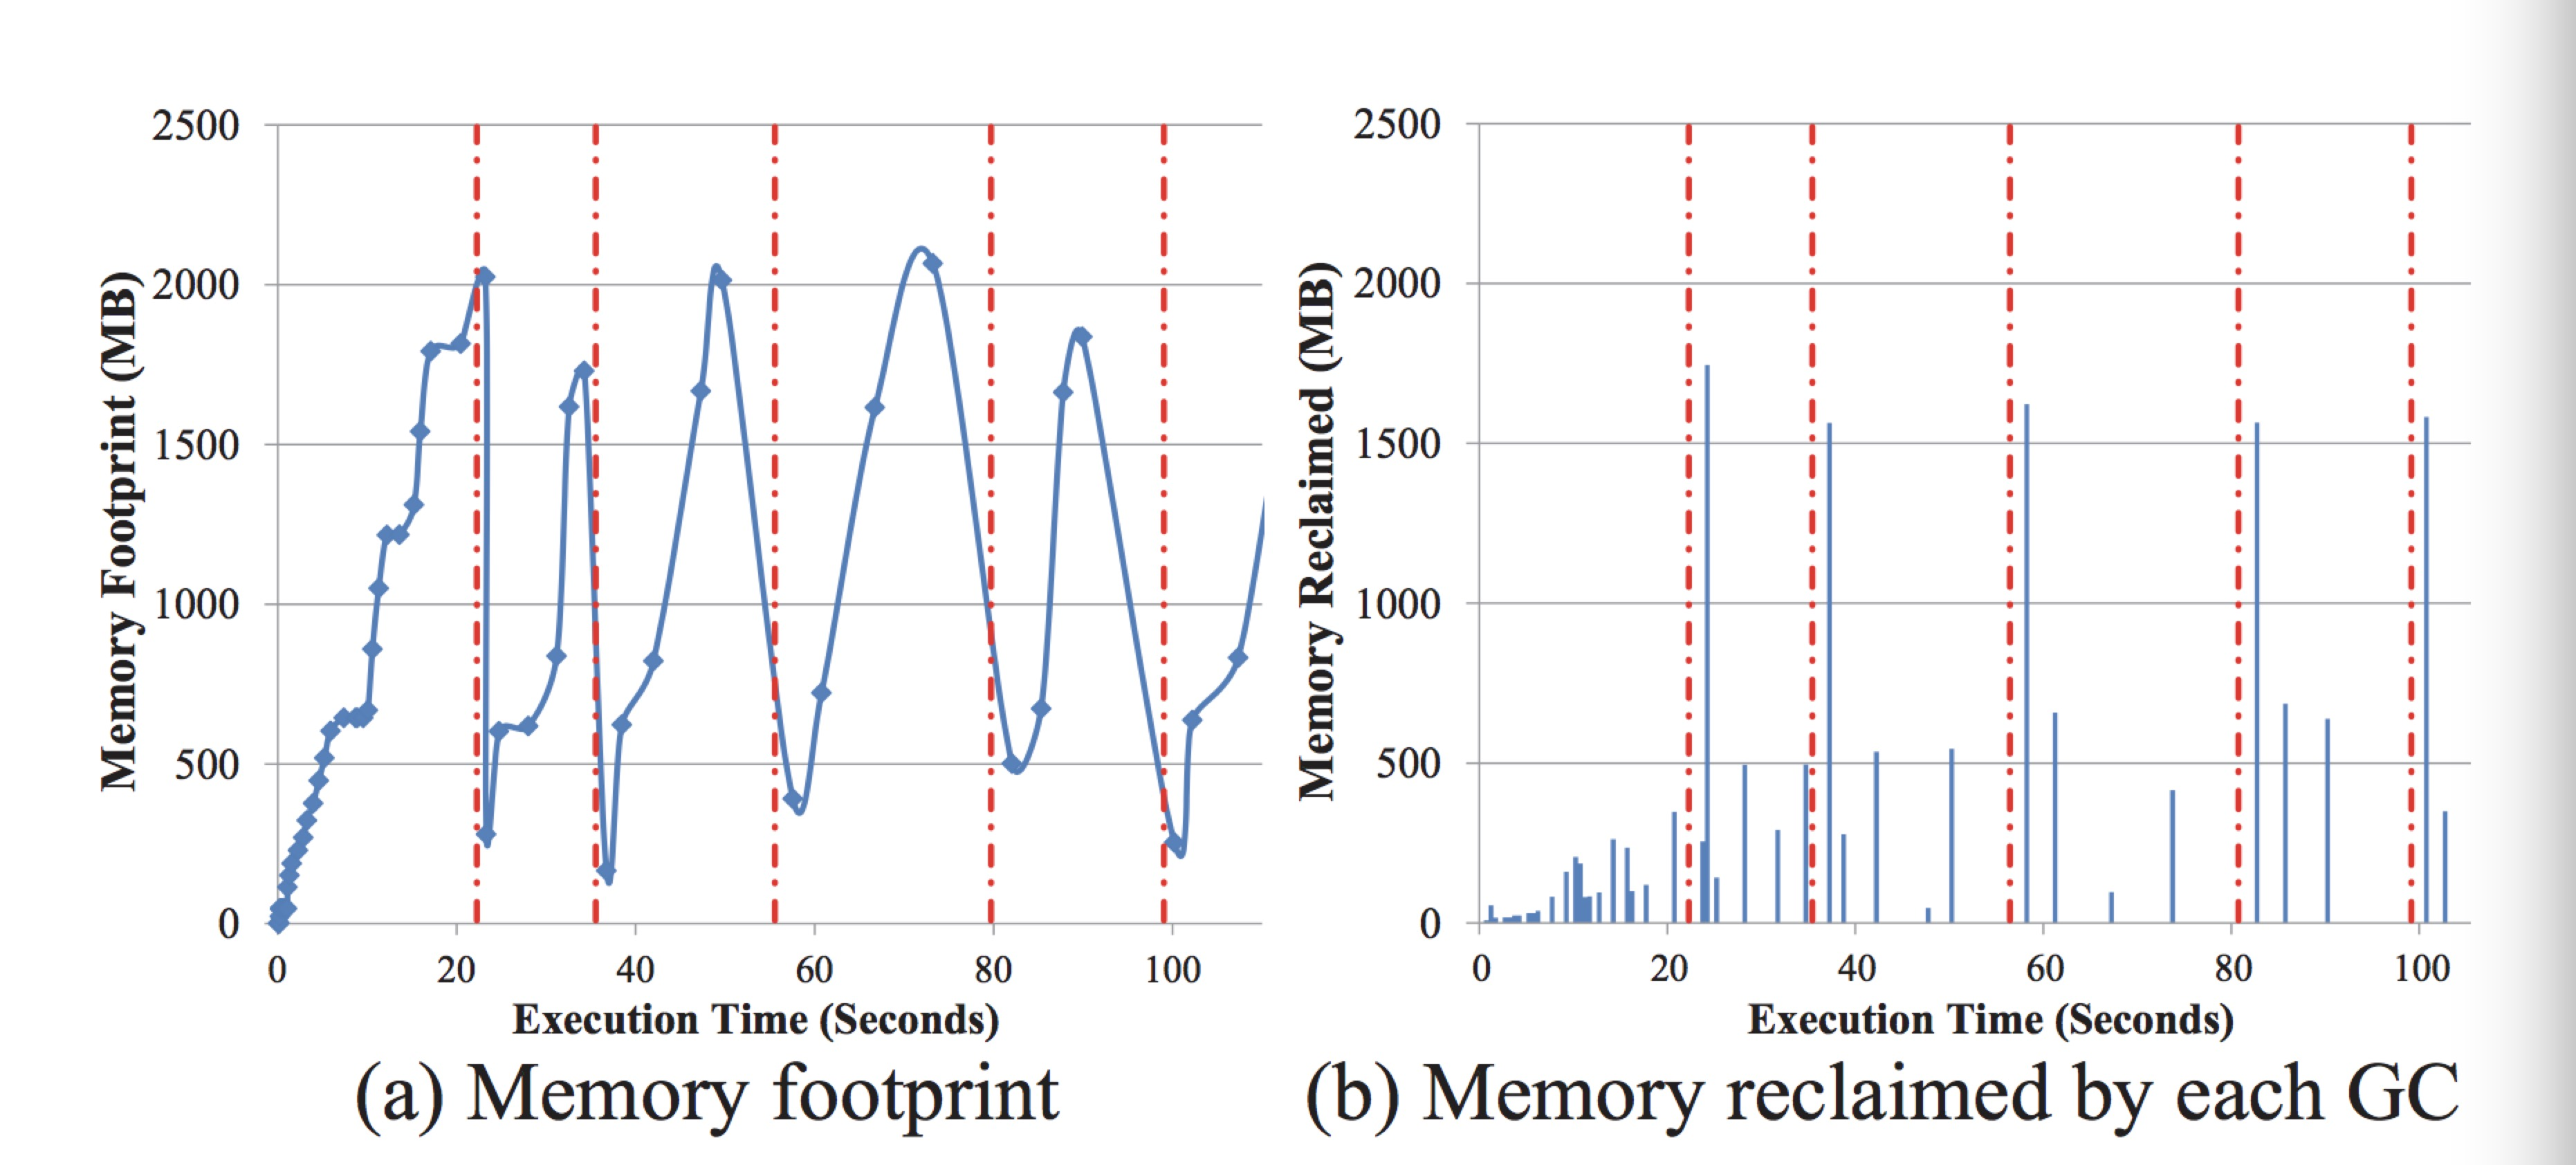
\includegraphics[width=12cm,height=7cm]{figure/footprint1.jpg}
    \caption{
        GraphChi执行期间的内存足迹,横轴为执行时间(GC消耗73\%的运行时间)。(a)中的每个点表示一次GC后对内存的测量,(b)中每条线显示每次GC回收内存数量;垂直虚线表示时域界限。
    }
    \label{footprint1}
\end{figure}

Yak性能好坏,很大程度上取决于大数据框架的对象特征与假设中时域特征的契合程度,以下是GraphChi程序的运行足迹。

在GraphChi实验中,GC占据73\%的运行时间。每个时域持续约20秒(虚线表示)。如\ref{footprint1}所示。我们可以观察到时域结束点和内存下降存在明显的相关性。在每个时域执行期间,GC运行但只能回收很少的内存,是一种资源的浪费 (\ref{footprint1}(b)),而在每个时域结束后,大量对象生命周期同时结束,这时执行GC,可以回收足够的内存。

\begin{figure}[h]
    \centering
    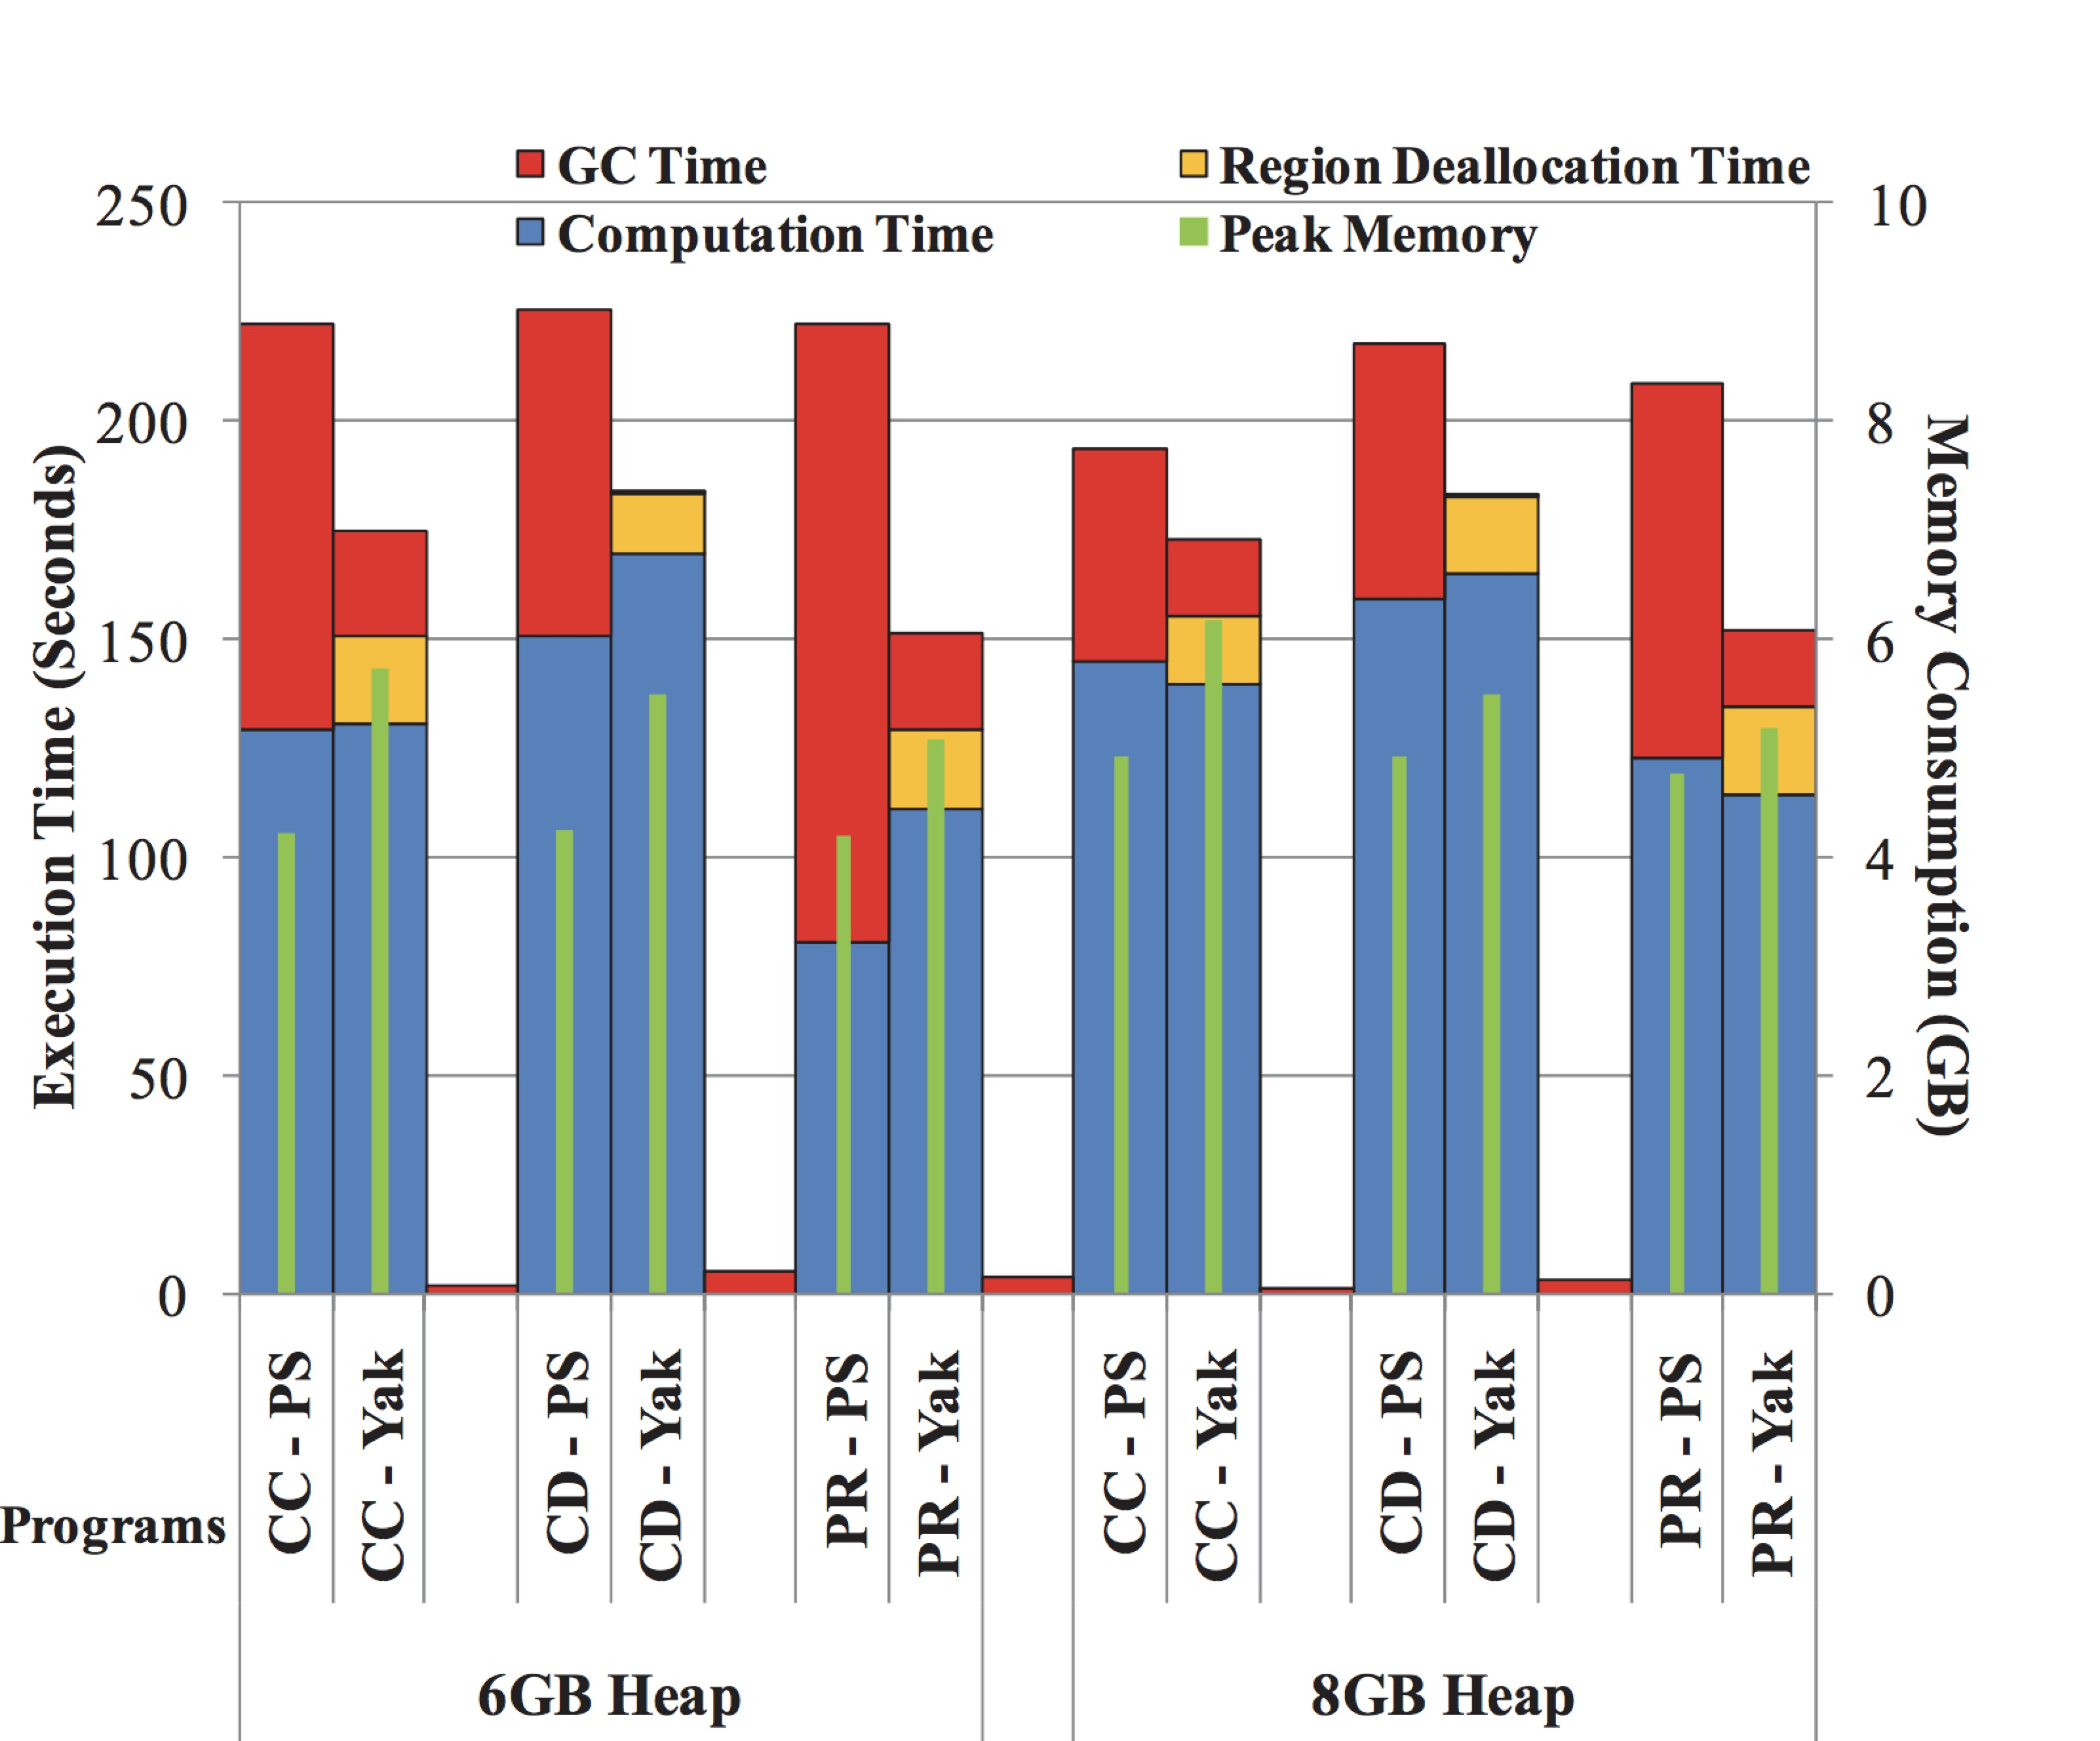
\includegraphics[width=12cm,height=7cm]{figure/evaluation1.jpg}
    \caption{
        Yak与Parallel Scavenge 在GraphChi不同程序执行时间的对比。堆内存分配分别为6GB和8GB。
    }
    \label{evaluation1}
\end{figure}

因为GraphChi对象具有强烈的时域特征,Yak在GraphChi上性能优势明显,如图\ref{evaluation1},对比Parallel Scavenge,Yak平均执行时间降低15\%。

作者在三种大数据框架——Hyracks、Hadoop、GraphChi都进行了实验,获得了显著的性能提升。

\begin{figure}[h]
    \centering
    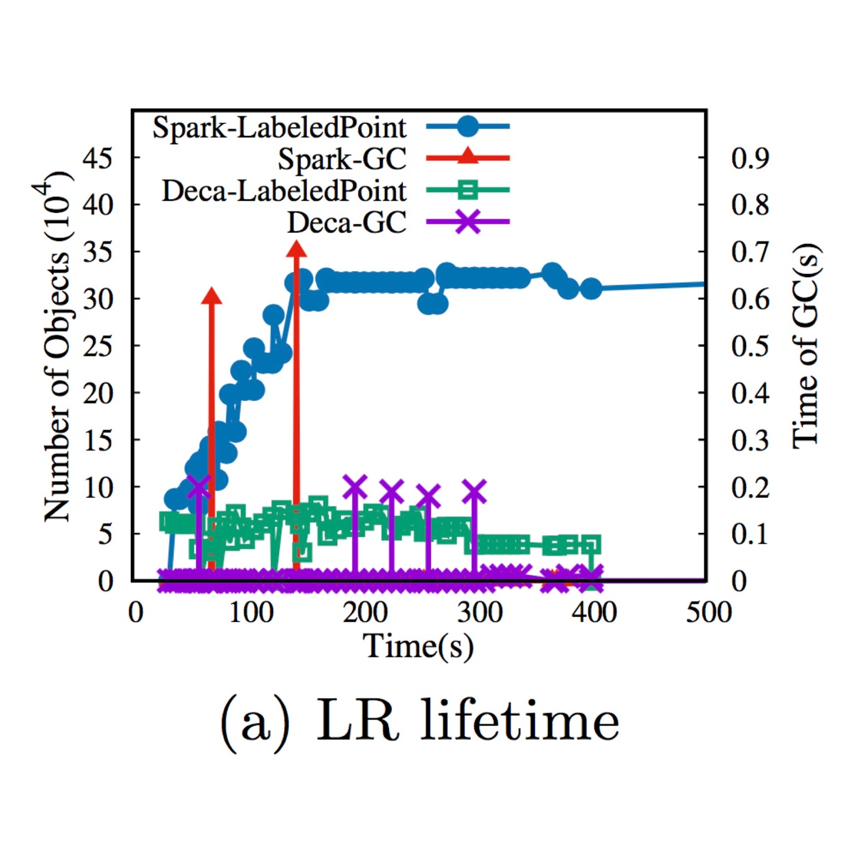
\includegraphics[width=12cm,height=9cm]{figure/evaluation2.png}
    \caption{
        Spark执行LR期间的内存足迹,横轴为执行时间,(a)中的每个点表示一次GC后对内存的测量。
    }
    \label{evaluation2}
\end{figure}
但是, Yak对时域(region)的粗粒度划分导致Yak适用的局限性,只有严格满足对象时域特征的数据框架才能较好地发挥Yak优势,epoch假设不适用于Spark等内存计算系统。Spark LR执行的过程中,每一次GC均会回收较多的无用数据,图\ref{evaluation2}是在spark中执行LR(Line Regression)内存的足迹,epoch假设不适用于Spark等内存计算系统。Spark的内存足迹没有显示出明显的时域界限,对象不满足严格的时域特征,Yak的内存回收方式不合适。

Yak粗粒度的时域划分导致系统性能与大数据框架中对象epoch特征紧密相关,当大数据框架中的对象epoch特征不明显时,Yak性能下降。

针对以上的缺陷,我们设想添加额外的、定义良好的细粒度时域来改善性能。

\subsection{低并行性}

Yak没有实现并行的原因就是在遇到多目的地问题时,必须严格按照拓扑排序迁移,所以整个迁移过程必须是串行的。

改进的思路是,我们可以在迁移前先进行完整的可达性分析,对含有相同对象的可达路径进行聚类,形成多个GC Task。Task内部可能存在多目的地问题,因此仍旧需要按照拓扑排序串行执行;而两个Task之间不存在交集,因此可以并行地执行对象迁移和引用更新,这样就可以提供一定的并行度,进一步优化GC性能。具体优化方案将在第五章讲解。

